\documentclass[11pt,]{article}
\usepackage[]{mathpazo}
\usepackage{amssymb,amsmath}
\usepackage{ifxetex,ifluatex}
\usepackage{fixltx2e} % provides \textsubscript
\ifnum 0\ifxetex 1\fi\ifluatex 1\fi=0 % if pdftex
  \usepackage[T1]{fontenc}
  \usepackage[utf8]{inputenc}
\else % if luatex or xelatex
  \ifxetex
    \usepackage{mathspec}
  \else
    \usepackage{fontspec}
  \fi
  \defaultfontfeatures{Ligatures=TeX,Scale=MatchLowercase}
\fi
% use upquote if available, for straight quotes in verbatim environments
\IfFileExists{upquote.sty}{\usepackage{upquote}}{}
% use microtype if available
\IfFileExists{microtype.sty}{%
\usepackage{microtype}
\UseMicrotypeSet[protrusion]{basicmath} % disable protrusion for tt fonts
}{}
\usepackage[margin=1in]{geometry}
\usepackage{hyperref}
\hypersetup{unicode=true,
            pdftitle={Supplement for: Multicentre validation of the CamGFR model for estimated glomerular filtration rate},
            pdfkeywords={Glomerular Filtration Rate, CamGFR, CKD-EPI, Carboplatin},
            pdfborder={0 0 0},
            breaklinks=true}
\urlstyle{same}  % don't use monospace font for urls
\usepackage{graphicx,grffile}
\makeatletter
\def\maxwidth{\ifdim\Gin@nat@width>\linewidth\linewidth\else\Gin@nat@width\fi}
\def\maxheight{\ifdim\Gin@nat@height>\textheight\textheight\else\Gin@nat@height\fi}
\makeatother
% Scale images if necessary, so that they will not overflow the page
% margins by default, and it is still possible to overwrite the defaults
% using explicit options in \includegraphics[width, height, ...]{}
\setkeys{Gin}{width=\maxwidth,height=\maxheight,keepaspectratio}
\IfFileExists{parskip.sty}{%
\usepackage{parskip}
}{% else
\setlength{\parindent}{0pt}
\setlength{\parskip}{6pt plus 2pt minus 1pt}
}
\setlength{\emergencystretch}{3em}  % prevent overfull lines
\providecommand{\tightlist}{%
  \setlength{\itemsep}{0pt}\setlength{\parskip}{0pt}}
\setcounter{secnumdepth}{0}
% Redefines (sub)paragraphs to behave more like sections
\ifx\paragraph\undefined\else
\let\oldparagraph\paragraph
\renewcommand{\paragraph}[1]{\oldparagraph{#1}\mbox{}}
\fi
\ifx\subparagraph\undefined\else
\let\oldsubparagraph\subparagraph
\renewcommand{\subparagraph}[1]{\oldsubparagraph{#1}\mbox{}}
\fi

%%% Use protect on footnotes to avoid problems with footnotes in titles
\let\rmarkdownfootnote\footnote%
\def\footnote{\protect\rmarkdownfootnote}

%%% Change title format to be more compact
\usepackage{titling}

% Create subtitle command for use in maketitle
\newcommand{\subtitle}[1]{
  \posttitle{
    \begin{center}\large#1\end{center}
    }
}

\setlength{\droptitle}{-2em}

  \title{Supplement for: Multicentre validation of the CamGFR model for estimated
glomerular filtration rate}
    \pretitle{\vspace{\droptitle}\centering\huge}
  \posttitle{\par}
    \author{}
    \preauthor{}\postauthor{}
    \date{}
    \predate{}\postdate{}
  
\usepackage{booktabs}
\usepackage{longtable}
\usepackage{array}
\usepackage{multirow}
\usepackage[table]{xcolor}
\usepackage{wrapfig}
\usepackage{float}
\usepackage{colortbl}
\usepackage{pdflscape}
\usepackage{tabu}
\usepackage{threeparttable}
\usepackage{threeparttablex}
\usepackage[normalem]{ulem}
\usepackage{makecell}

\newcommand{\beginsupplement}{\setcounter{table}{0} \renewcommand{\thetable}{S\arabic{table}} \setcounter{figure}{0} \renewcommand{\thefigure}{S\arabic{figure}}} \usepackage{breqn} \usepackage{biblatex} \usepackage{graphicx} \usepackage{textgreek}

\begin{document}
\maketitle
\begin{abstract}
This document is a supplemental file for the paper ``Multicentre
validation of the CamGFR model for estimated glomerular filtration
rate'' and provides additional methods, results, figures and tables. The
.Rmd file format contains the R code used for this manuscript and is
available at
\href{https://github.com/EdwardHWilliams/CamGFRValidationNonIDMS}{github.com/EdwardHWilliams/CamGFRValidationNonIDMS}.
\end{abstract}

\beginsupplement

\section{Data description and
filtering}\label{data-description-and-filtering}

Raw data that were received from the seven different centres, which are
identified by their location (Cambridge, Edinburgh, London-Barts,
Manchester, Melbourne, Southampton and Wales). Data were individually
processed and cleaned prior to being used for analyses. This step
involved exploring the data for manual transcription errors such as the
height and weight variable being swapped and removing unrealistic values
for some variables. During this process all data were converted to the
same units to enable data pooling and analyses across the different
centres and subgroup categories.

Next, patients with data outside the inclusion criteria were removed.
The inclusion criteria were:

\begin{itemize}
\item Serum creatinine value between 18 \textmu mol/L (0.2 mg/dL) and 400 \textmu mol/L (4.5 mg/dL)
\item Age of 18 years or older
\item Creatinine and GFR measurements performed within 30 days of each other 
\end{itemize}

The creatinine cut-off values were chosen because the lower value is the
typical detection threshold on the measurement assay and the upper value
is 3-4 times the upper limit of normal in most centres, thus
corresponding to a value at which most clinicians would consider kidney
function severely impaired.

All creatinine data were either measured using a non-IDMS traceable
measurement or the measurement procedure was not known. Table
\ref{tab:creat_info} summarises the information on the creatinine
measurement for each centre.

\begin{table}[H]
\caption{Creatinine methods used at each centre}
\begin{tabular}{|l|l|l|}
\hline
\textbf{Centre} & \textbf{Date range}                                                           & \textbf{Creatinine measurment method}                                                                                                                                                                                               \\ \hline 

Cambridge       & 2013                                                                          & Dimension RxL compensated Jaffe, not IDMS-traceable                                                                                                                                                                                                                  \\ \hline
Edinburgh       & 2011 - 2017                                                                   & \begin{tabular}[c]{@{}l@{}}An Abbott Architect assay using the Jaffe method;  \\ 
not IDMS-traceable \end{tabular}                                                                                             \\ \hline
London-Barts    & 2010 - 2017                                                                   & Unknown method; IDMS usage not known                                                                                                                                                                                                                  \\ \hline
Manchester      & 2012 - 2016                                                                   & \begin{tabular}[c]{@{}l@{}} Jaffe method  using O’Leary reagent; \\
not IDMS-tracable  \end{tabular}                                                                                                                                                          \\ \hline
Melbourne       & 2000 - 2005                                                                   & Jaffe method; not IDMS-traceable \\ \hline
Southampton     & 1999 - 2012                                                                   & \begin{tabular}[c]{@{}l@{}}Jaffe method; given the date range, most, \\
if not all, not IDMS-traceable\end{tabular}                                                                \\ \hline
Wales           & \begin{tabular}[c]{@{}l@{}}2005 - 2011, \\ not all dates\\ known\end{tabular} & \begin{tabular}[c]{@{}l@{}}Different centres used either Jaffe or enzymatic methods; \\ 
IDMS usage not known\end{tabular} \\ \hline
\end{tabular}
\label{tab:creat_info}
\end{table}

Table 1 in the main manuscript provides the number of patients in
different categorical groups and the summary statistics for the
continuous variables (GFR, age, serum creatinine, body surface area
(BSA), height and weight) for all patients. Here we provide the summary
statistics for patients split into different centres (Table
\ref{tab:summary_centre}).

\begin{longtable}[t]{lrrrrrrr}
\caption{\label{tab:print_data_characteristic_tables}\label{tab:summary_centre}Summary characteristics for patients from each centre separately}\\
\toprule
  & Mean & SD & Minimim & Q1 & Median & Q3 & Maximum\\
\midrule
\endfirsthead
\caption[]{\label{tab:summary_centre}Summary characteristics for patients from each centre separately \textit{(continued)}}\\
\toprule
  & Mean & SD & Minimim & Q1 & Median & Q3 & Maximum\\
\midrule
\endhead
\
\endfoot
\bottomrule
\endlastfoot
\addlinespace[0.6em]
\multicolumn{8}{l}{\textbf{Cambridge}}\\
\hline
\hspace{1em}GFR [ml/min] & 86 & 29 & 9 & 65 & 85 & 105 & 211\\
\hspace{1em}Creatinine [µmol/L] & 87 & 27 & 40 & 70 & 83 & 97 & 258\\
\hspace{1em}Age [years] & 55 & 16 & 18 & 44 & 56 & 67 & 86\\
\hspace{1em}Weight [kg] & 77 & 19 & 39 & 64 & 74 & 87 & 184\\
\hspace{1em}Height [cm] & 169 & 10 & 146 & 161 & 168 & 177 & 200\\
\hspace{1em}BSA [m²] & 1.86 & 0.24 & 1.34 & 1.69 & 1.85 & 2.01 & 2.87\\
\addlinespace[0.6em]
\multicolumn{8}{l}{\textbf{Edinburgh}}\\
\hline
\hspace{1em}GFR [ml/min] & 83.7 & 34.9 & 9.1 & 54.6 & 83 & 110.2 & 206\\
\hspace{1em}Creatinine [µmol/L] & 90 & 32 & 45 & 70 & 81 & 102 & 393\\
\hspace{1em}Age [years] & 56 & 16 & 18 & 43 & 58 & 68 & 87\\
\hspace{1em}Weight [kg] & 79 & 19 & 38 & 66 & 78 & 90 & 197\\
\hspace{1em}Height [cm] & 171 & 10 & 144 & 164 & 171 & 179 & 202\\
\hspace{1em}BSA [m²] & 1.91 & 0.24 & 1.27 & 1.73 & 1.91 & 2.06 & 3.17\\
\addlinespace[0.6em]
\multicolumn{8}{l}{\textbf{London-Barts}}\\
\hline
\hspace{1em}GFR [ml/min] & 110 & 20 & 46 & 98 & 111 & 122 & 166\\
\hspace{1em}Creatinine [µmol/L] & 81 & 14 & 52 & 73 & 82 & 88 & 141\\
\hspace{1em}Age [years] & 39.2 & 9.2 & 22.4 & 32.7 & 38.7 & 45.1 & 70.8\\
\hspace{1em}Weight [kg] & 85 & 17 & 57 & 73 & 82 & 90 & 150\\
\hspace{1em}Height [cm] & 177.9 & 7.8 & 160 & 172.8 & 177.8 & 182 & 200\\
\hspace{1em}BSA [m²] & 2 & 0.2 & 1.6 & 1.9 & 2 & 2.1 & 2.6\\
\addlinespace[0.6em]
\multicolumn{8}{l}{\textbf{Manchester}}\\
\hline
\hspace{1em}GFR [ml/min] & 77 & 29 & 14 & 56 & 74 & 94 & 194\\
\hspace{1em}Creatinine [µmol/L] & 88 & 22 & 46 & 74 & 83 & 96 & 235\\
\hspace{1em}Age [years] & 62 & 14 & 18 & 54 & 65 & 72 & 91\\
\hspace{1em}Weight [kg] & 72 & 19 & 33 & 59 & 70 & 83 & 164\\
\hspace{1em}Height [cm] & 164.6 & 9.8 & 137 & 157 & 164 & 171 & 200\\
\hspace{1em}BSA [m²] & 1.78 & 0.24 & 1.17 & 1.6 & 1.76 & 1.93 & 2.79\\
\addlinespace[0.6em]
\multicolumn{8}{l}{\textbf{Melbourne}}\\
\hline
\hspace{1em}GFR [ml/min] & 85 & 31 & 17 & 64 & 83 & 104 & 205\\
\hspace{1em}Creatinine [µmol/L] & 96 & 30 & 60 & 80 & 90 & 110 & 290\\
\hspace{1em}Age [years] & 63 & 13 & 18 & 56 & 65 & 72 & 87\\
\hspace{1em}Weight [kg] & 73 & 15 & 37 & 62 & 72 & 80 & 145\\
\hspace{1em}Height [cm] & 169.4 & 9.3 & 148 & 163 & 170 & 176.6 & 194\\
\hspace{1em}BSA [m²] & 1.83 & 0.21 & 1.31 & 1.69 & 1.83 & 1.96 & 2.62\\
\addlinespace[0.6em]
\multicolumn{8}{l}{\textbf{Southampton}}\\
\hline
\hspace{1em}GFR [ml/min] & 119 & 21 & 51 & 104 & 118 & 132 & 209\\
\hspace{1em}Creatinine [µmol/L] & 89 & 12 & 54 & 80 & 89 & 97 & 136\\
\hspace{1em}Age [years] & 39.9 & 9.5 & 19 & 33 & 39 & 46 & 75\\
\hspace{1em}Weight [kg] & 86 & 16 & 54 & 76 & 85 & 95 & 200\\
\hspace{1em}Height [cm] & 179 & 7 & 156 & 174 & 179 & 183 & 204\\
\hspace{1em}BSA [m²] & 2.05 & 0.19 & 1.62 & 1.92 & 2.03 & 2.16 & 3.09\\
\addlinespace[0.6em]
\multicolumn{8}{l}{\textbf{Wales}}\\
\hline
\hspace{1em}GFR [ml/min] & 89 & 31 & 23 & 65 & 90 & 111 & 169\\
\hspace{1em}Creatinine [µmol/L] & 74 & 19 & 38 & 61 & 74 & 84 & 164\\
\hspace{1em}Age [years] & 57 & 18 & 22 & 42 & 58 & 72 & 90\\
\hspace{1em}Weight [kg] & 77 & 18 & 45 & 63 & 76 & 88 & 155\\
\hspace{1em}Height [cm] & 168 & 11 & 145 & 160 & 166 & 177 & 192\\
\hspace{1em}BSA [m²] & 1.86 & 0.24 & 1.41 & 1.67 & 1.83 & 2.04 & 2.57\\*
\end{longtable}

\begin{table}

\caption{\label{tab:print_data_diagnosis}\label{tab:summary_diagnosis}Number of patients with given diagnoses in each centre}
\centering
\resizebox{\linewidth}{!}{
\begin{tabular}[t]{l|r|r|r|r|r|r|r|r}
\hline
Diagnosis & Manchester & Edinburgh & Cambridge & Southampton & Melbourne & Wales & London-Barts & Total\\
\hline
\multicolumn{9}{l}{\textbf{Cancer}}\\
\hline
\hspace{1em}GCT & 35 & 118 & 58 & 436 & 0 & 67 & 108 & 822\\
\hline
\hspace{1em}Unknown & 437 & 8 & 48 & 0 & 308 & 0 & 0 & 801\\
\hline
\hspace{1em}Gynae & 251 & 54 & 104 & 0 & 0 & 89 & 0 & 498\\
\hline
\hspace{1em}Bladder/TCC & 88 & 138 & 26 & 0 & 0 & 0 & 0 & 252\\
\hline
\hspace{1em}Thoracic & 219 & 13 & 4 & 0 & 0 & 0 & 0 & 236\\
\hline
\hspace{1em}Gastro-oesophageal & 203 & 19 & 5 & 0 & 0 & 0 & 0 & 227\\
\hline
\hspace{1em}Head and Neck & 192 & 3 & 6 & 0 & 0 & 0 & 0 & 201\\
\hline
\hspace{1em}Endometrial & 104 & 21 & 0 & 0 & 0 & 0 & 0 & 125\\
\hline
\hspace{1em}Uterus/Cervix & 83 & 15 & 1 & 0 & 0 & 0 & 0 & 99\\
\hline
\hspace{1em}Sarcoma & 31 & 36 & 12 & 0 & 0 & 0 & 0 & 79\\
\hline
\hspace{1em}Breast & 29 & 6 & 2 & 0 & 0 & 0 & 0 & 37\\
\hline
\hspace{1em}HPB & 26 & 6 & 0 & 0 & 0 & 0 & 0 & 32\\
\hline
\hspace{1em}Colorectal & 17 & 10 & 0 & 0 & 0 & 0 & 0 & 27\\
\hline
\hspace{1em}CUP & 26 & 1 & 0 & 0 & 0 & 0 & 0 & 27\\
\hline
\hspace{1em}RCC & 12 & 6 & 0 & 0 & 0 & 0 & 0 & 18\\
\hline
\hspace{1em}Prostate & 5 & 8 & 0 & 0 & 0 & 0 & 0 & 13\\
\hline
\hspace{1em}Neuroendocrine & 1 & 11 & 0 & 0 & 0 & 0 & 0 & 12\\
\hline
\hspace{1em}Anal & 6 & 1 & 0 & 0 & 0 & 0 & 0 & 7\\
\hline
\hspace{1em}CNS & 6 & 0 & 0 & 0 & 0 & 0 & 0 & 6\\
\hline
\hspace{1em}Skin & 5 & 0 & 0 & 0 & 0 & 0 & 0 & 5\\
\hline
\hspace{1em}Melanoma & 1 & 0 & 0 & 0 & 0 & 0 & 0 & 1\\
\hline
\multicolumn{9}{l}{\textbf{Haematological}}\\
\hline
\hspace{1em}Haematological & 0 & 22 & 114 & 0 & 0 & 0 & 0 & 136\\
\hline
\multicolumn{9}{l}{\textbf{Non-cancer}}\\
\hline
\hspace{1em}\hspace{1em}Kidney donor & 0 & 94 & 35 & 0 & 0 & 0 & 0 & 129\\
\hline
\hspace{1em}Transplant & 0 & 0 & 28 & 0 & 0 & 0 & 0 & 28\\
\hline
\hspace{1em}Unknown & 0 & 9 & 0 & 0 & 0 & 0 & 0 & 9\\
\hline
\end{tabular}}
\end{table}

To facilitate data comparison graphically, Figure
\ref{fig:centre_boxplot} displays the data from Table
\ref{tab:summary_centre} in several boxplots. Patients from Southampton
and London-Barts have a higher GFR, height and weight and a lower age
than patients from other centres. This is attributable to the fact that
the data from these centres were from patients with seminoma only and
hence were typically from young men. The panel of log(creatinine)
illustrates the inter-centre variability.

\begin{figure}
\centering
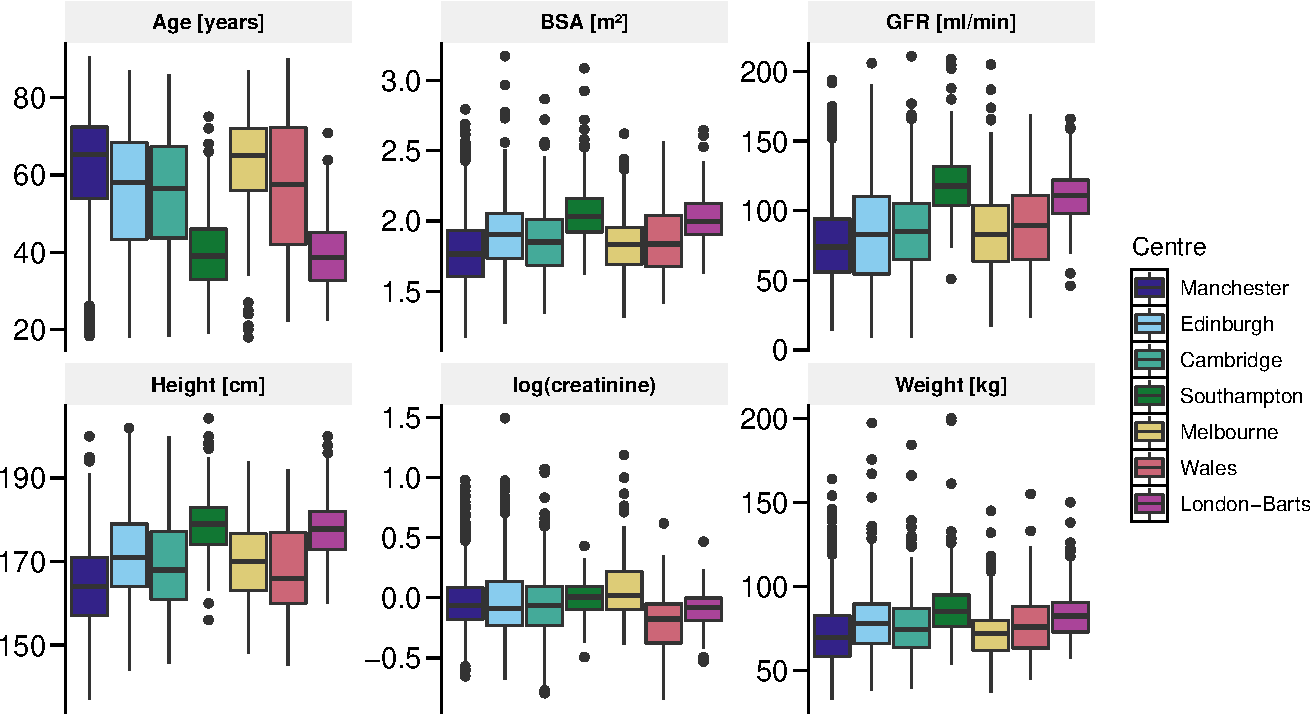
\includegraphics{1_Validation_nonIDMS_files/figure-latex/data_characteristics_plot_1-1.pdf}
\caption{\label{fig:centre_boxplot}Boxplot of the continuous variables
split by centre. Creatinine has been log transformed.}
\end{figure}

Figure \ref{fig:boxplot_creat} show boxplots for log(creatinine) split
by centre for all patients and patients with selected diagnoses
respectively. As patients with similar diagnoses should be approximately
matched for the other variables, the plots facilitate further comparison
of serum creatinine differences between centres.

\begin{figure}
\centering
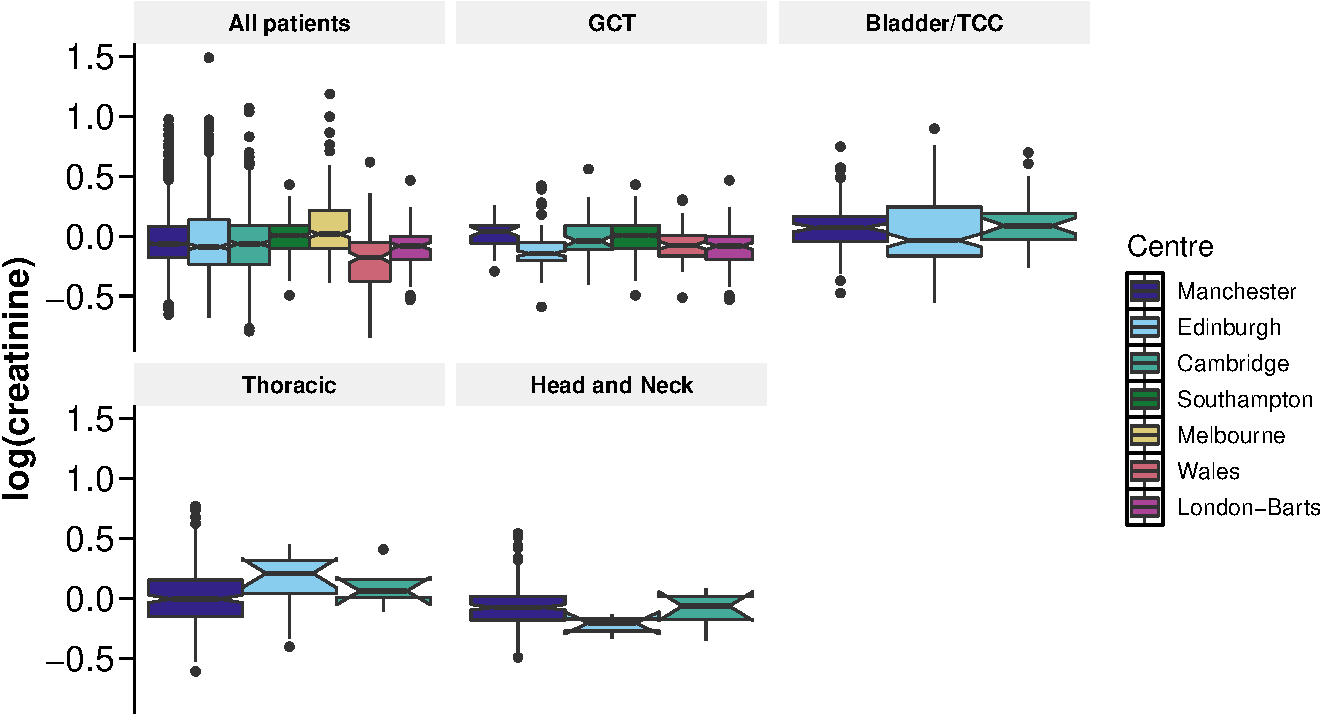
\includegraphics{1_Validation_nonIDMS_files/figure-latex/PLOT_analyse_creatinine-1.pdf}
\caption{\label{fig:boxplot_creat}Boxplots of the serum creatinine of
patients from different centres. Boxplots are shown for all patients
combined and for patients with Germ Cell Tumours (GCT), Bladder or
Transitional cell cancer (TCC), Thoracic cancer, Gastro-oesophageal
cancer and Head and Neck cancer. The notches in the boxplots are
\(1.58 \text{IQR} / \sqrt{n}\) (where \(n\) is the number of patient
used for the given boxplot and IQR is the inter quartile range); they
provide both an approximate 95\% confidence interval for the median and
an indication of the number of patients used for the given boxplot.}
\end{figure}

Figure \ref{fig:boxplot_diagnosis} takes the same format as Figure
\ref{fig:centre_boxplot} but displays subgroups of patients based on
diagnosis. Subgroups with more than 50 patients were included.

\begin{figure}
\centering
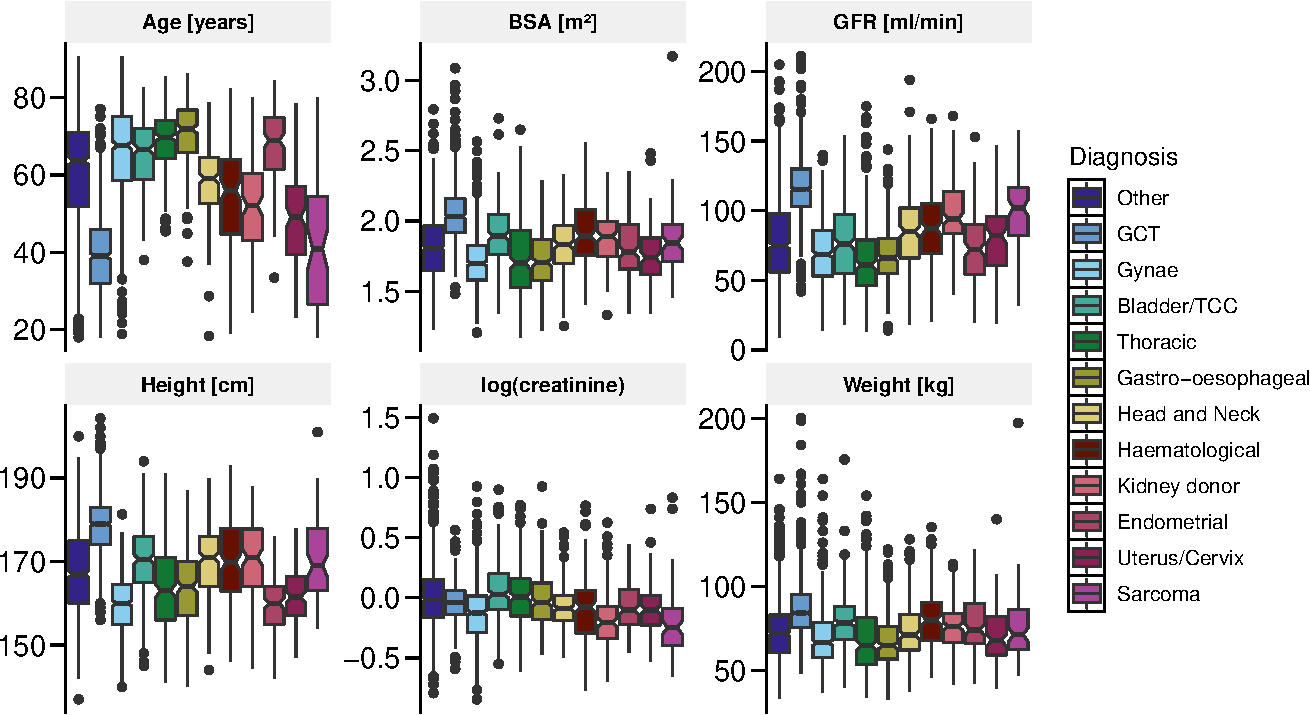
\includegraphics{1_Validation_nonIDMS_files/figure-latex/data_characteristics_plots_2-1.pdf}
\caption{\label{fig:boxplot_diagnosis}Boxplot of the continuous
variables split by diagnosis. Subgroups with more than 50 patients are
displayed. Subgroups with fewer than 50 patients have been combined with
patients with an unknown diagnosis into the group Other. Boxplots are
arranged by decreasing patient numbers from left to right. Serum
creatinine has been log transformed.}
\end{figure}

Information on ethnicity was available for patients from Cambridge and
Manchester, who comprised the majority of patients. From a total of
2,055 patients with known ethnicity, 1,947 were White (either White
British, White Irish, White other), 71 were Asian (Asian Indian, Asian
Pakistani, Asian Bangladeshi, Asian other, Chinese, Other Chinese, Mixed
White and Asian), 22 were Black (Black African, Black Caribbean, Black
other, Mixed White and Black Caribbean, Mixed White and Black African)
and 15 were of other ethnicity (other ethnic group, other mixed). Figure
\ref{fig:boxplot_race} shows boxplots for age, BSA, mGFR and
log(creatinine) for patients from the ethnic subgroups. As white
patients were the largest subgroup, t-tests were performed to look for
differences between this subgroup and each other subgroup. There were no
significant differences in the serum creatinine levels for patients from
different ethnicities. However, there were significant differences in
the other variables and therefore the subgroups were not matched. Given
the correlations between these variables, it is difficult to interpret
the creatinine comparisons precisely. To determine whether the average
creatinine values differ between white and black patients when the other
variables are similar, we sampled 22 white patients from the population
that matched the set of black patients with regards to sex and age ten
times. We then performed t-tests for these ten samples for
log(creatinine), measured GFR and BSA. No significant differences were
found (Table \ref{tab:race_resample}).

\begin{figure}
\centering
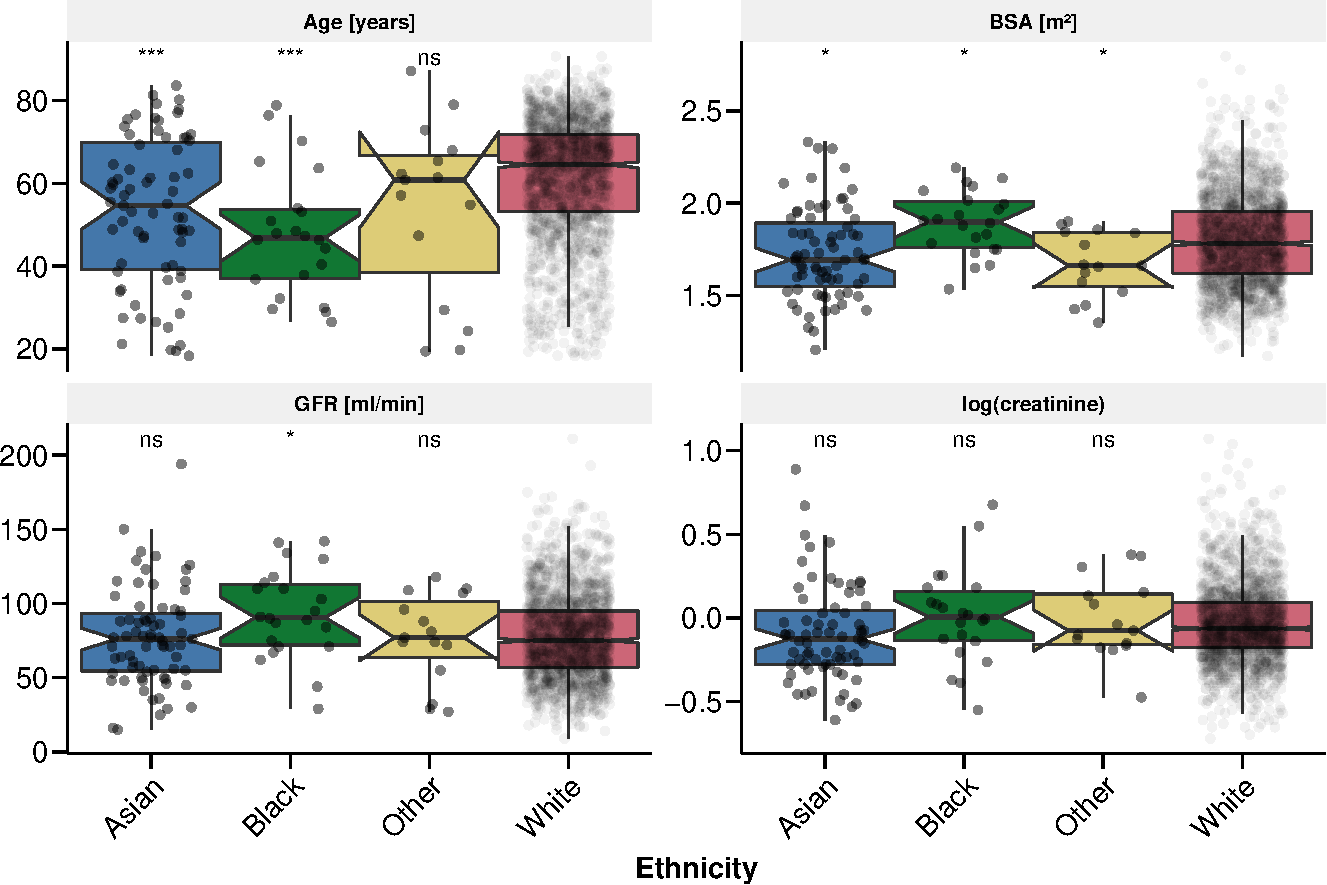
\includegraphics{1_Validation_nonIDMS_files/figure-latex/Ethnicity_boxplot-1.pdf}
\caption{\label{fig:boxplot_race}Boxplots of age, BSA, GFR and
log(creatinine) and Age where patients are split by ethnicity. The `*'
or `ns' at the top of the boxplot represents the p-value from a t-test
between the largest subgroup of white patients and each other ethnic
subgroups, where `ns' represents a p-value greater than 0.05 and `*',
`**' and `***' represent p-values less than 0.05, 0.01 and 0.001
respectively.}
\end{figure}

\begin{table}

\caption{\label{tab:ethnicity_matched_sampling}\label{tab:race_resample}t-test p-values for comparing the mean age, log(creatinine), GFR and BSA between 22 patients who were ethnically black and 22 random patients who were ethnically white and matched by mean age (mean age within 1 year) and the same gender distribution (12 females and 10 males).}
\centering
\begin{tabular}[t]{r|r|r|r}
\hline
Age [years] & log(creatinine) & GFR [ml/min] & BSA [m²]\\
\hline
0.98 & 0.39 & 0.72 & 0.88\\
\hline
0.92 & 0.29 & 0.61 & 0.16\\
\hline
0.93 & 0.01 & 0.98 & 0.06\\
\hline
0.89 & 0.89 & 0.91 & 0.93\\
\hline
0.91 & 0.51 & 0.92 & 0.57\\
\hline
0.90 & 0.53 & 0.59 & 0.83\\
\hline
0.85 & 0.67 & 0.79 & 0.88\\
\hline
0.86 & 0.44 & 0.74 & 0.78\\
\hline
0.97 & 0.31 & 0.65 & 0.68\\
\hline
0.94 & 0.38 & 0.10 & 0.19\\
\hline
\end{tabular}
\end{table}

\section{Comparison of models}\label{comparison-of-models}

We compared the CamGFR\textsuperscript{1} model with the the following
published models: CKD-EPI\textsuperscript{2}, MDRD (186
version)\textsuperscript{3}, Wright\textsuperscript{4},
Cockcroft-Gault\textsuperscript{5}, Jelliffe\textsuperscript{6},
Mayo\textsuperscript{7} and Martin\textsuperscript{8}. If these
equations estimated BSA-normalised GFR (CKD-EPI, MDRD, Jelliffe and
Mayo), the estimated value was subsequently unnormalised by multiplying
the estimated value by \(1.73/\textrm{BSA}\), where \(\textrm{BSA}\) is
the patient's body surface area estimated using the DuBois-DuBois
equation:
\[\textrm{BSA} = 0.20247 \times \textrm{Height}^{0.725} \times \textrm{Weight}^{0.425}\]
where height is measured in metres and weight is measured in kg. Some of
these models (Cockroft-Gault and Jelliffe) were developed to estimate
creatinine clearance and not GFR, where creatinine clearance is itself a
biased estimator of GFR. These models are included as they are still
used to estimate GFR by some centres, clinical trial groups, and in
other settings.

The equations were compared using three metrics: the
root-mean-squared-error (RMSE), median residual value, and the residual
interquartile range (IQR). These three metrics are estimators for a
model's accuracy, bias and precision respectively. A 95\% confidence
interval was calculated for each of these metrics using the bootstrap
resampling procedure. Specifically, 2,000 resamples with replacement
(where the sample size was the same as the number of data points) were
taken from the data used to calculate the metric. The metric was then
calculated for each of these 2,000 samples and using the normal
approximation a confidence interval was constructed\textsuperscript{9}.
The seed was reset to be the same when sampling the 2,000 replicates for
the different metrics.

The main results of this analysis are reported in Figure 1 (results for
patients split by centre) in the main manuscript along with Figures
\ref{fig:performace_diagnosis} (results for patients split by
diagnosis), \ref{fig:performace_age} (results for patients split by age)
and \ref{fig:performace_BSA} (results for patients split by BSA).
Additionally, all numerical results are reported in Table S5 (an
additional file). Table S5 gives the results for all equations above
whereas the Figures only compare the performance of CamGFR, CKD-EPI,
MDRD, Wright and Cockroft-Gault.

\begin{figure}
\centering
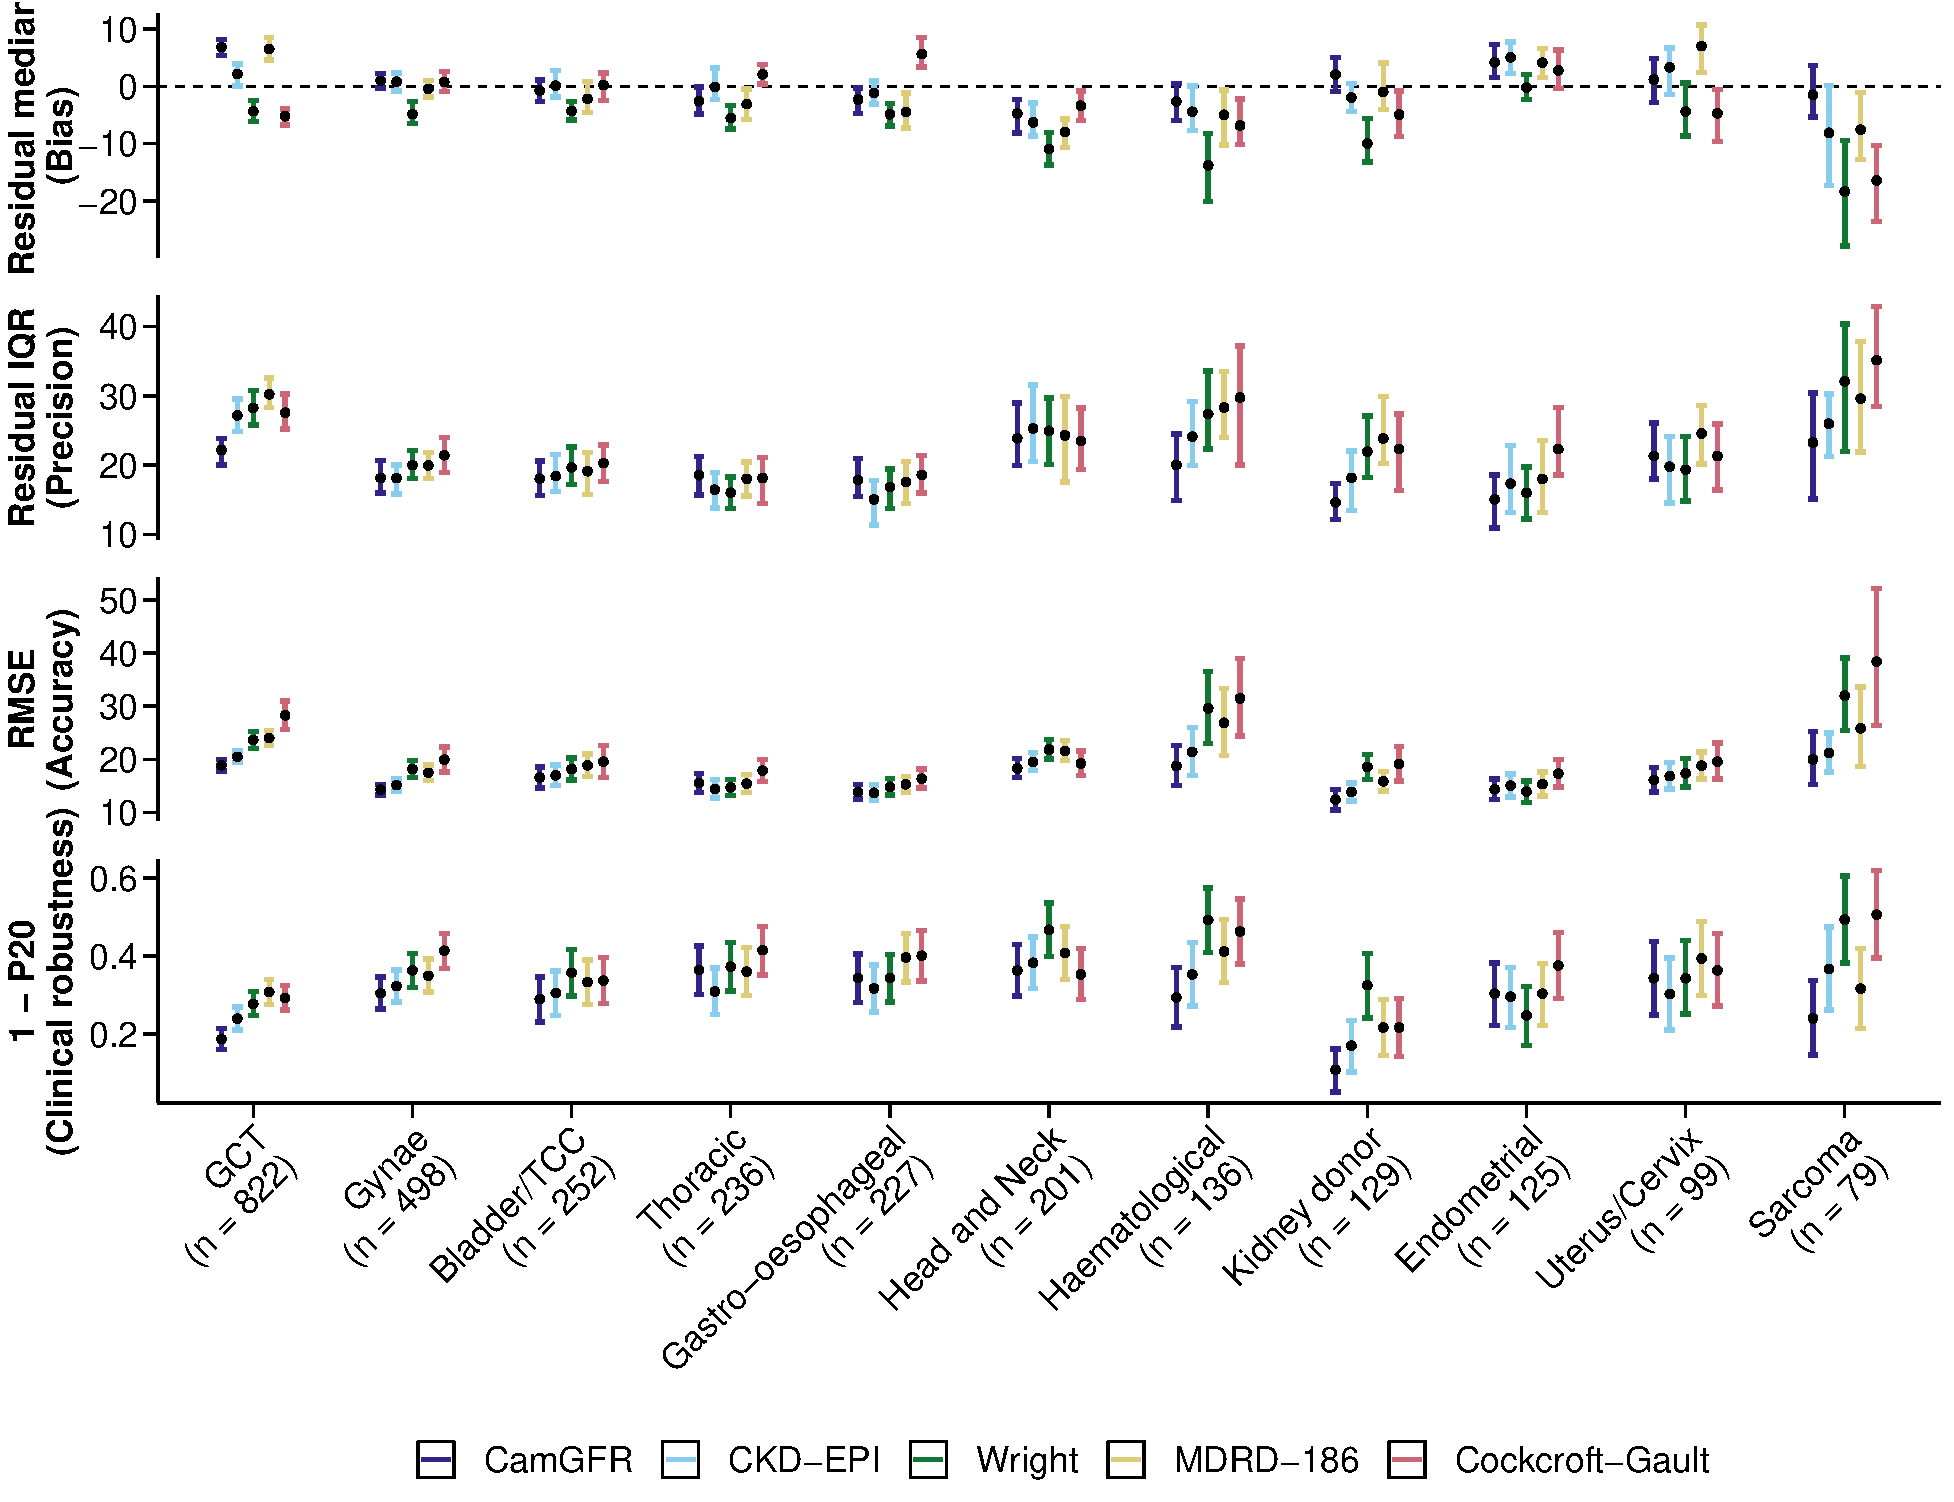
\includegraphics{1_Validation_nonIDMS_files/figure-latex/PLOT_dagnosis-1.pdf}
\caption{\label{fig:performace_diagnosis}Performance of GFR models for
patients from different diagnostic subgroups. The results for the CamGFR
model and four other commonly used other models (CKD-EPI, Wright,
MDRD-186 and Cockcroft-Gault) are displayed. Results for those
diagnostic subgroups that had more than 50 patients are shown. (first
row) The residual (measured GFR - estimated GFR) median, which is a
measure of a model's bias, is displayed. (second row) The residual
interquartile range (IQR), which is a measure of a model's precision, is
displayed. (third row) The root-mean-squared error (RMSE), which is a
measure of a model's accuracy, is displayed. Accuracy is a combination
metric of bias and precision. (fourth row) The proportion of patients
who have an absolute percentage error more than 20\% (1-P20), which
reflects clinical robustness by illustrating the proportion of patients
with a clinically relevant error, is displayed.The best result would be
closest to zero for the residual median, and the smallest value for IQR,
RMSE, and 1-P20. All error bars are 95\% confidence intervals calculated
using bootstrap resampling with 2,000 repetitions and a normal
distribution approximation.}
\end{figure}

We analysed performance when patients were split into groups by their
age or BSA. Figures \ref{fig:performace_age} and
\ref{fig:performace_BSA} show the performance of each model for equally
sized subgroups of age and BSA, respectively. The accuracy of all models
tends to increase with increasing age and tends to increase with
increasing BSA. These observations can be largely explained by the fact
that GFR is modelled on the square root scale in the CamGFR model and on
the log scale for the CKD-EPI or MDRD models. Patients who are young or
have a large BSA also tend to have a higher GFR and patients with a
higher GFR will have a less accurate estimated GFR due to modelling on a
square-root or log scale.

\begin{figure}
\centering
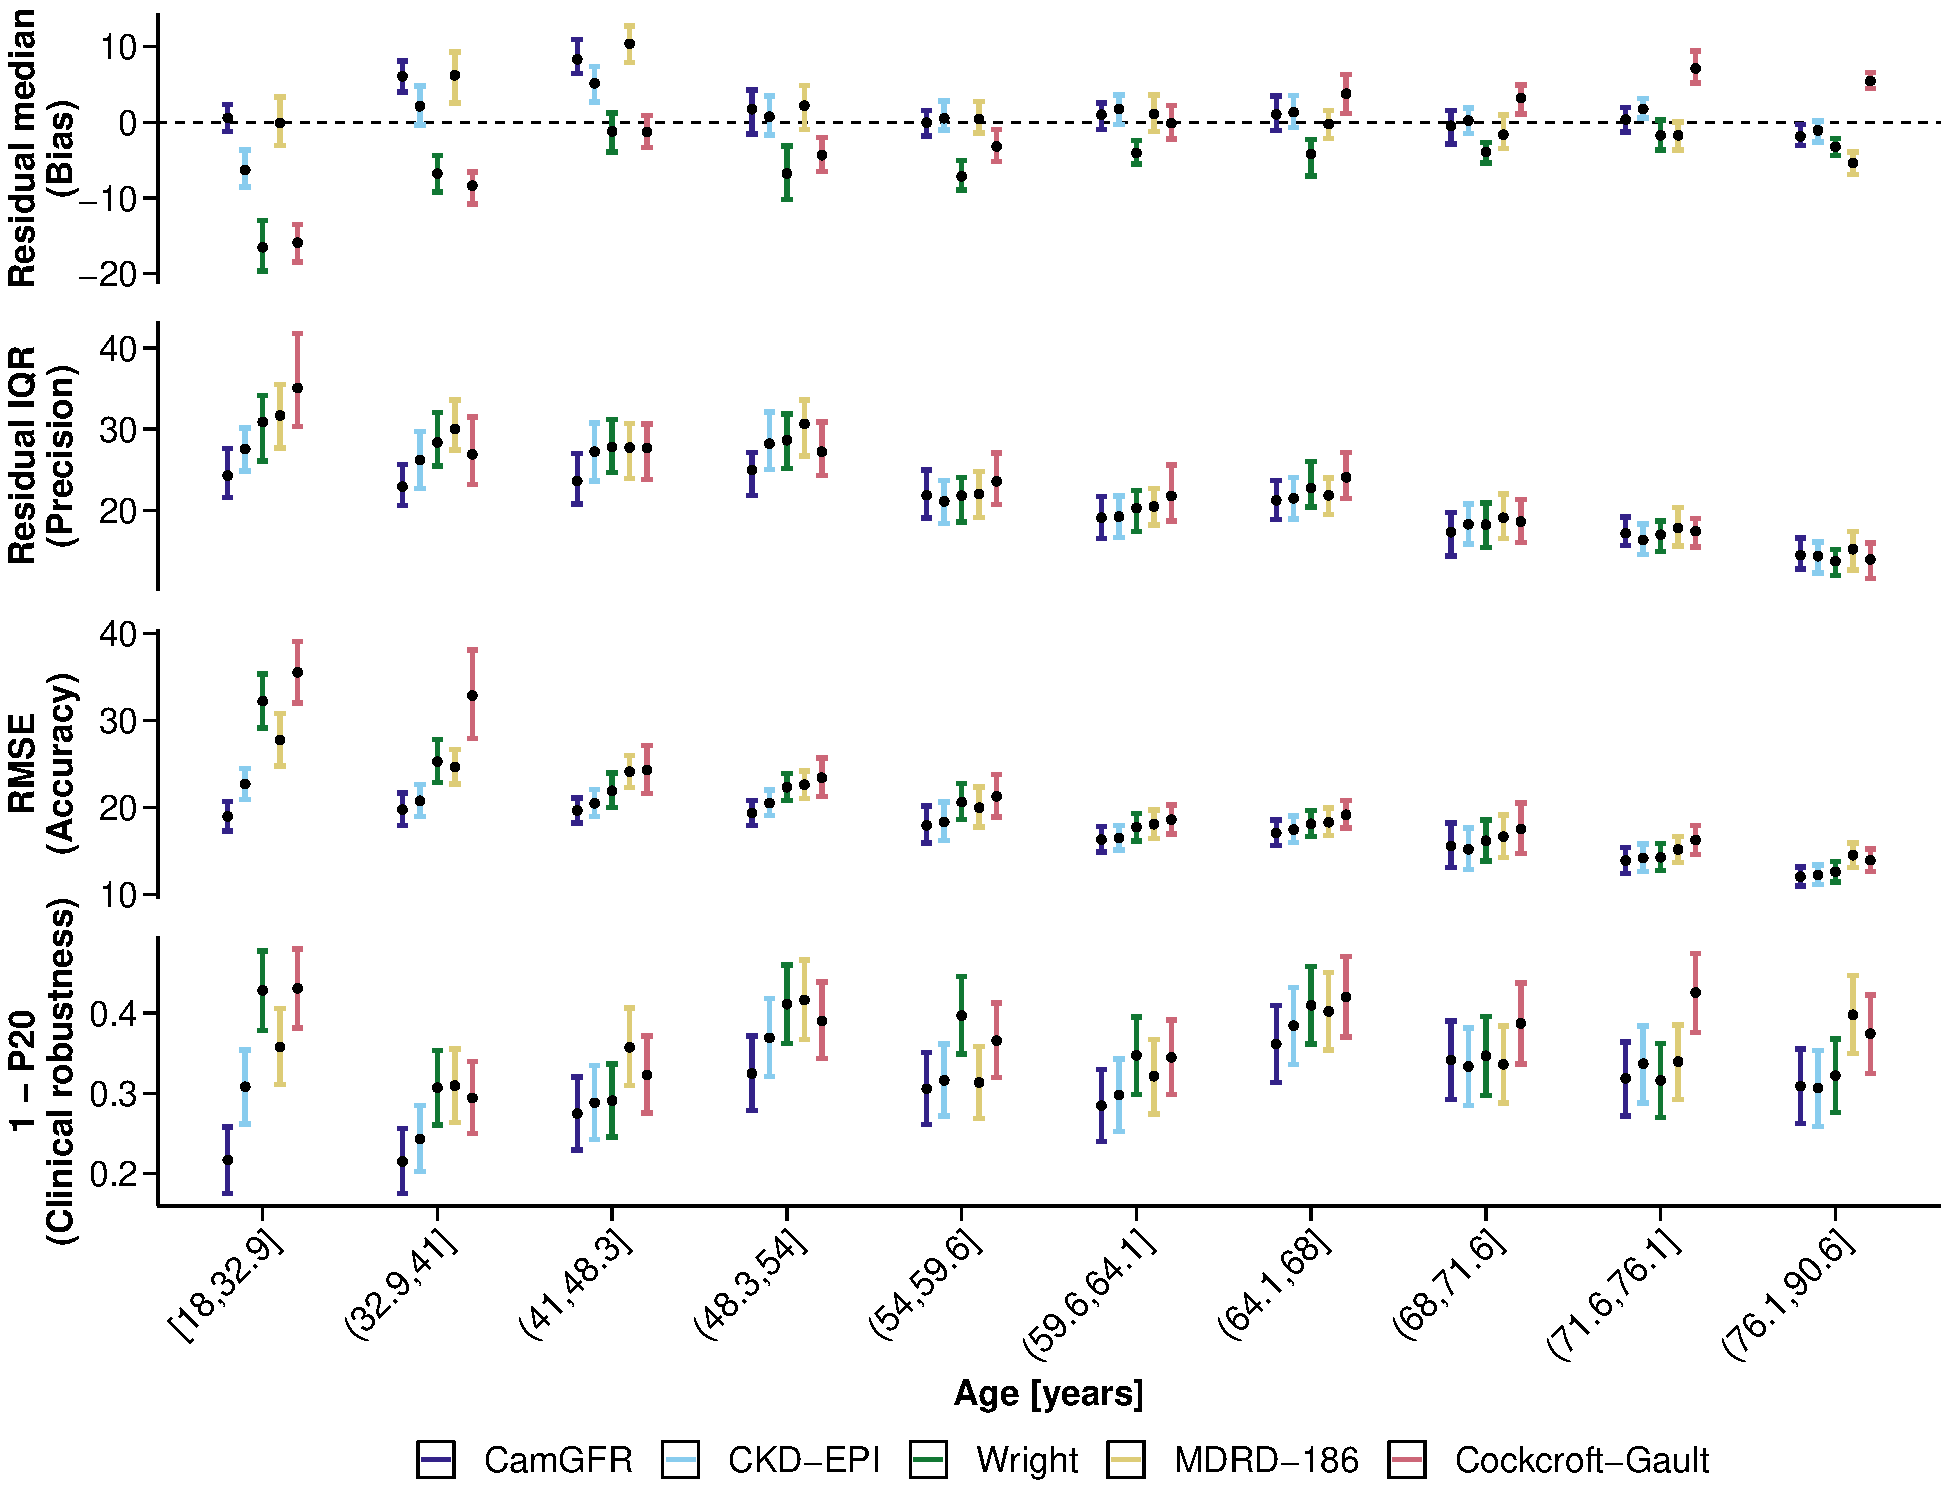
\includegraphics{1_Validation_nonIDMS_files/figure-latex/PLOT_performance_age-1.pdf}
\caption{\label{fig:performace_age}Comparison of model performance in
different age groups. The results for five published models are shown.
Patients were split into 10 equally sized groups by their age.
(\emph{a},\emph{b}{]} denotes the interval \emph{a} to \emph{b} which is
exclusive of the lower and inclusive of the higher age.}
\end{figure}

\begin{figure}
\centering
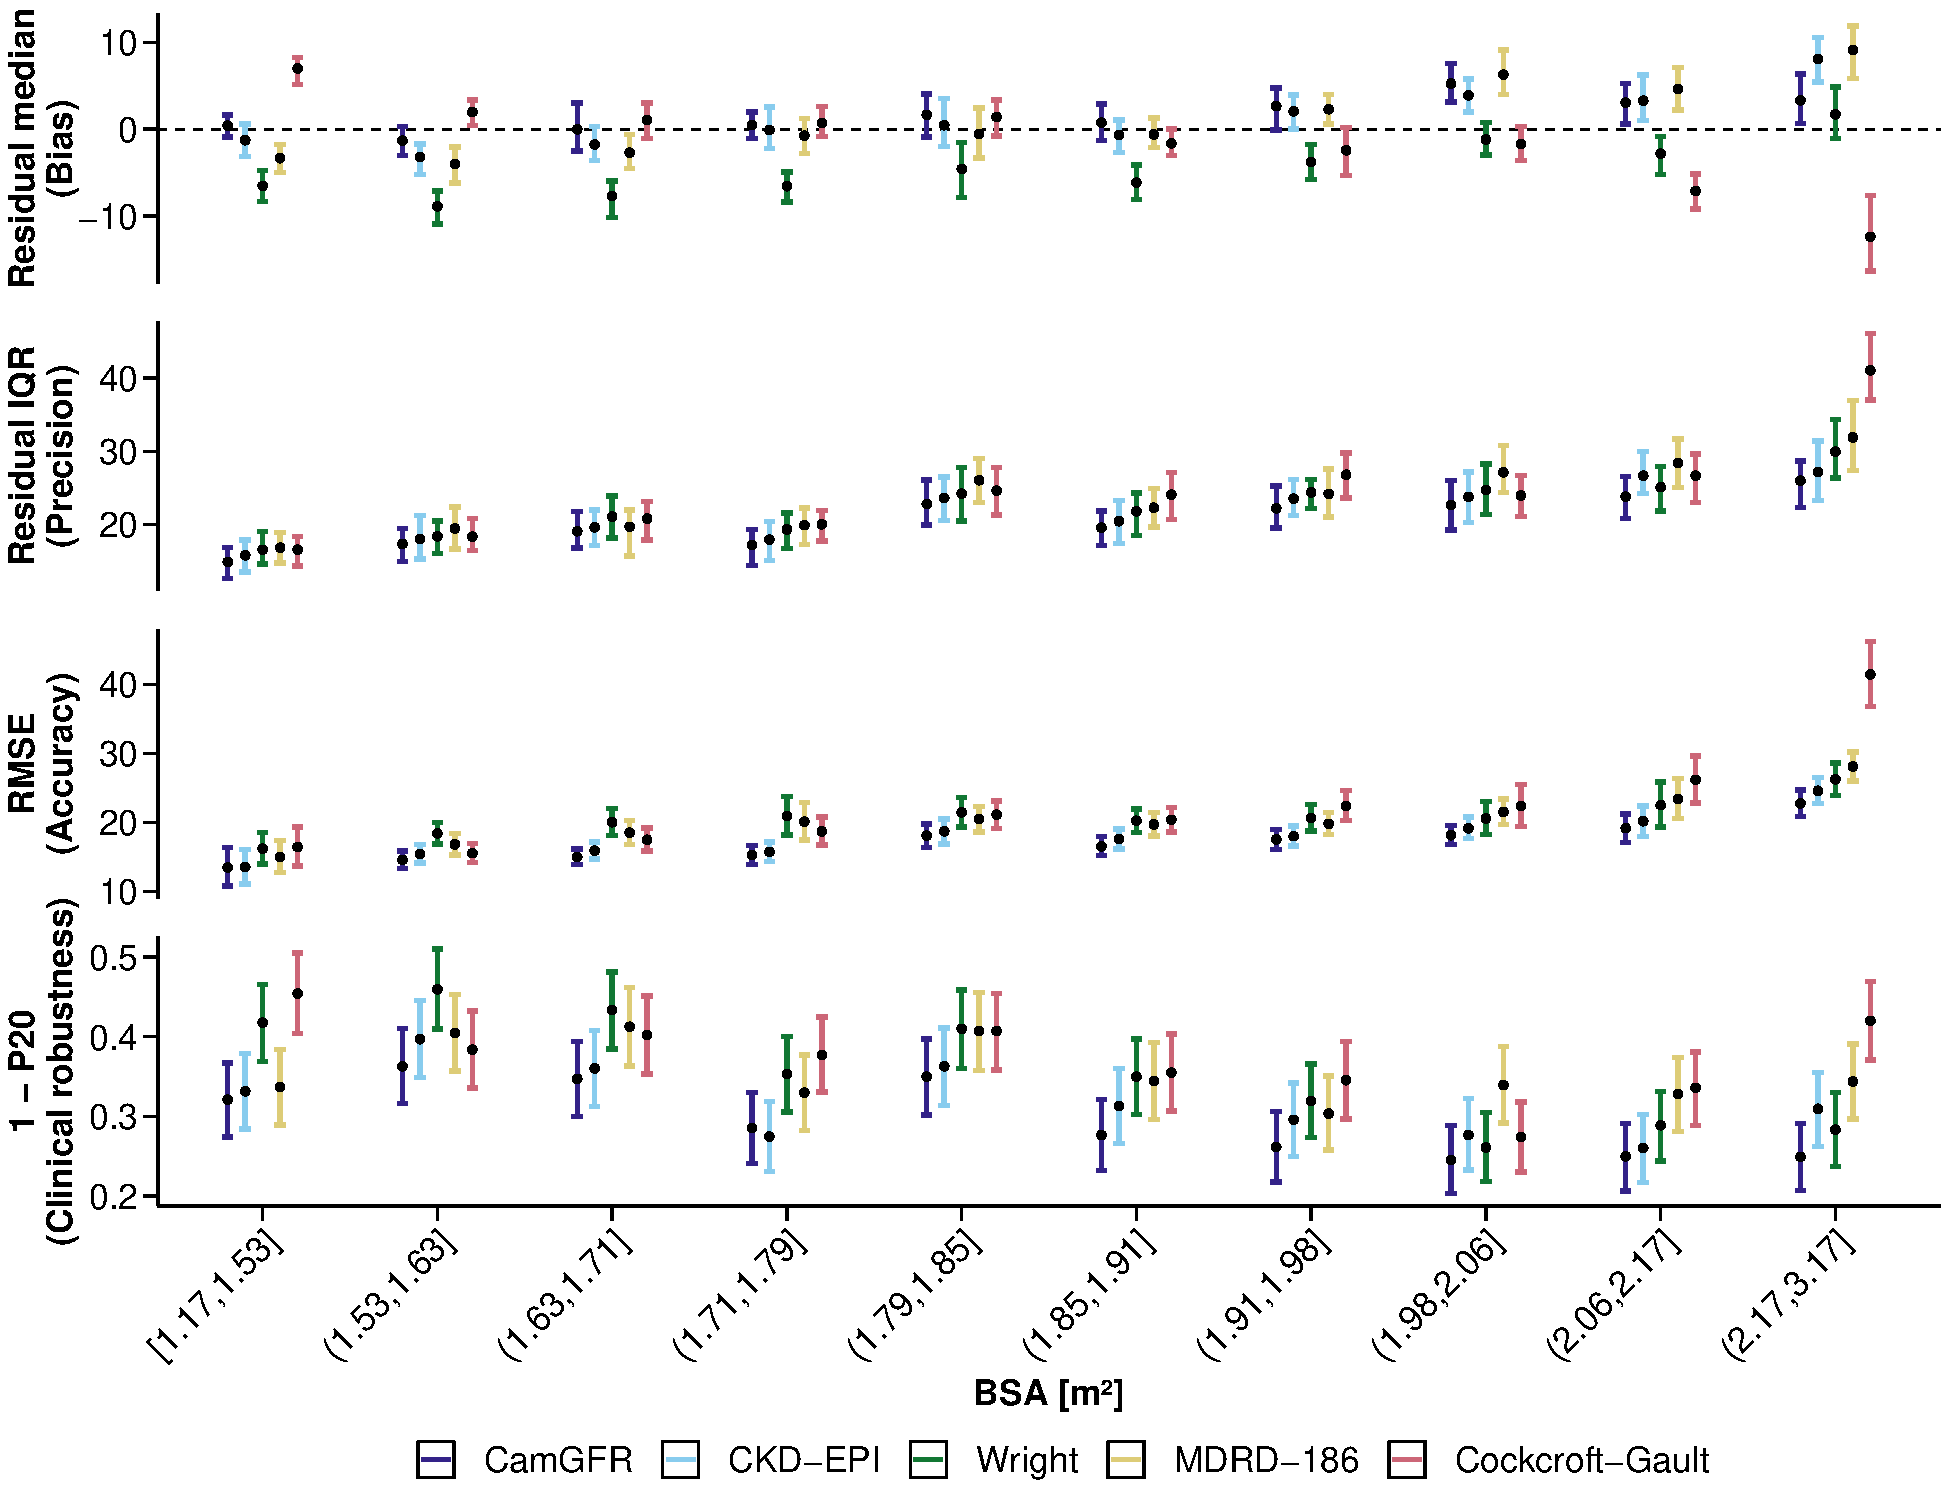
\includegraphics{1_Validation_nonIDMS_files/figure-latex/PLOT_performance_BSA-1.pdf}
\caption{\label{fig:performace_BSA}Comparison of model performance in
different BSA groups. The results for five published models are shown.
Patients were split into 10 equally sized groups by their BSA.
(\emph{a},\emph{b}{]} denotes the interval \emph{a} to \emph{b} which is
exclusive of the lower and inclusive of the higher BSA.}
\end{figure}

P-values for the differences between a statistic for a pair of equations
were calculated using a bootstrap procedure described by
Efron\textsuperscript{10}. In this procedure we have two samples
\(\mathbf{z}\) and \(\mathbf{y}\) of lengths \(n\) and \(m\)
respectively, from possibly different probability distributions \(F\)
and \(G\). In our case \(F\) and \(G\) were the probability
distributions of the residuals for the two equations of interest. We
tested the null hypothesis \(H_0: F = G\), against the alternative
hypothesis \(H_0: F \neq G\). Let \(x = [z,y]\), and chose a test
statistic \(t(\mathbf{x})\), which had the form
\(t(\mathrm{x}) = f(\mathrm{z}) - f(\mathrm{y})\), where the function
\(f(\mathrm{w})\) was either RMSE, median or IQR. Using the following
procedure an approximate p-value was calculated by:

\begin{itemize}
\item For $r = 1, ..., R$ let $\mathrm{x}^*_r$ be a sample with replacement of size $n+m$ from the pooled vector $\mathrm{x} = [\mathrm{z}, \mathrm{y}]$. Let $\mathrm{z}^*_r$ be the first $n$ observations of  $\mathrm{x}^*_r$ and $\mathrm{y}^*_r$ the remaining $m$ observations.
\item Let 
$$t_r^* = t(\mathrm{x}^*_r) = f(\mathrm{z}^*_r) - f(\mathrm{y}^*_r), \quad r = 1, 2, ..., R$$
\item Calculate the approximate p-value for the hypothesis test as: 
$$ \widehat{p} =\frac{1 + \sum_{r=1}^R \mathbb{1}_{\left| t_r^*\right| \geq \left| t_{obs}\right|}}{R + 1}$$ 
where $t_{obs} = t(\mathrm{x}) = f(\mathrm{z}) - f(\mathrm{y})$ is the observed value of the statistic and $\mathbb{1}_A$ is the indicator function which returns $1$ if $A$ is true and $0$ otherwise. The absolute values of $t$ are considered so as to perform a two-sided test. 
\end{itemize}

It should be noted that that the hypothesis test is strictly testing the
null hypothesis \(H_0 :F=G\) and not the null hypothesis
\(H_0: f(Z) = f(G)\). When the approximate p-values are calculated with
the statistic 1-P20 (the proportion of patients with an absolute
percentage error more than 20\%), \(z\) and \(y\) would be the vectors
of percentage differences between the fitted and measured dose values.
Approximate p-values (with \(R = 10,000\)) are given in Tabel S5 (an
additional file).

\section{Published models}\label{published-models}

This section gives the published models used in this manuscript. In the
following equations:

\begin{itemize}
\item $Age$ is the patient's Age in years
\item $BSA$ is the patient's body surface area in $m^2$, if is estimated for the patients weight and weight using the DuBois DuBois equation [@Janowitz2017a] 
\item $Scr$ is the patient's blood serum cratinine in $mg/dL$
\item $Wt$ is the patient's weight is $kg$
\end{itemize}

\subsection{\texorpdfstring{CamGFR\textsuperscript{1}}{CamGFR1}}\label{camgfr-janowitz2017a}

\begin{dmath*}
GFR = \left( 1.81395 + 0.01914\!\!\times\!\! Age  + 4.73278\!\!\times\!\! BSA - 0.02970 \!\!\times\!\! Age\!\!\times\!\! BSA - 3.71619\!\!\times\!\! \text{log}\left( Scr\right) + 1.06284 \!\!\times\!\! \text{log}\left( Scr\right)^2 -0.91420 \!\!\times\!\! \text{log}\left( Scr\right)^3 + \left( 0.02020 + 0.01247\!\!\times\!\! Age\right) \left[ \text{if male} \right] \right)^2
\end{dmath*}

\subsection{\texorpdfstring{CKD-EPI\textsuperscript{2}}{CKD-EPI2}}\label{ckd-epi-levey2009}

\begin{equation*}
GFR = \begin{cases}
141\times \text{min}\left(\frac{Scr}{0.7}, 1\right)^{-0.329} \times \text{max}\left(\frac{Scr}{0.7}, 1\right)^{-1.209} \times Age^{0.993} \times 1.018 & \text{if Sex = F} \\
141\times \text{min}\left(\frac{Scr}{0.9}, 1\right)^{-0.411} \times \text{max}\left(\frac{Scr}{0.9}, 1\right)^{-1.209} \times Age^{0.993}  & \text{if Sex = M}
      \end{cases}
\end{equation*}

\subsection{\texorpdfstring{Cockcroft
Gault\textsuperscript{5}}{Cockcroft Gault5}}\label{cockcroft-gault-cockcroft1976}

\begin{equation*}
 GFR = \frac{(140-Age) \times Wt \times (1-0.15[\text{if female}])}{72\times Scr}
\end{equation*}

\subsection{\texorpdfstring{MDRD-186\textsuperscript{3}}{MDRD-1863}}\label{mdrd-186-levey2016}

\begin{equation*}
GFR = 186 \times Scr^{-1.154} \times Age^{-0.203} \times 0.742 [\text{if female}]
\end{equation*}

\subsection{\texorpdfstring{Jelliffe\textsuperscript{6}}{Jelliffe6}}\label{jelliffe-jelliffe1973}

\begin{equation*}
GFR = \frac{(98-0.8(Age-20))\times(1-0.1[\text{if female}])\times \frac{BSA}{1.73}}{Scr}
\end{equation*}

\subsection{\texorpdfstring{Wright\textsuperscript{4}}{Wright4}}\label{wright-wright2001a}

\begin{equation*}
GFR = \frac{(6580-38.8\times Age)\times(1-0.168[\text{if female}])\times BSA}{88.42*Scr}
\end{equation*}

\subsection{\texorpdfstring{Mayo
Quadratic\textsuperscript{7}}{Mayo Quadratic7}}\label{mayo-quadratic-rule2004}

\begin{equation*}
GFR = \exp \left(1.911 + 5.249\frac{1}{Scr} - 2.114\frac{1}{Scr^2} - 0.00686Age - 0.205 [\text{if female}]\right)
\end{equation*}

if \(Scr < 0.8\)mg/dL then use \(0.8\) for \(Scr\)

\subsection{\texorpdfstring{Martin\textsuperscript{8}}{Martin8}}\label{martin-martin1998}

\begin{equation*}
GFR = \frac{163\times \mathrm{Wt}\ \times(1-0.00496\times \mathrm{Age})\times(1-0.252[\text{if female}])}{88.42\times \mathrm{Scr}}
\end{equation*}

\section*{References}\label{references}
\addcontentsline{toc}{section}{References}

\hypertarget{refs}{}
\hypertarget{ref-Janowitz2017a}{}
1. Janowitz T, Williams EH, Marshall A, et al. New model for estimating
glomerular filtration rate in patients with cancer. \emph{Journal of
Clinical Oncology : official journal of the American Society of Clinical
Oncology}. 2017;35(24):2798-2805.
doi:\href{https://doi.org/10.1200/JCO.2017.72.7578}{10.1200/JCO.2017.72.7578}

\hypertarget{ref-Levey2009}{}
2. Levey AS, Stevens LA, Frcp C, et al. A new equation to estimate
glomerular filtration rate. \emph{Annals of Internal Medicine}.
2009;150(9):604-612.
doi:\href{https://doi.org/10.7326/0003-4819-150-9-200905050-00006}{10.7326/0003-4819-150-9-200905050-00006}

\hypertarget{ref-Levey2016}{}
3. Levey AS, Bosch JP, Lewis JB, Greene T. A more accurate method to
estimate glomerular filtration rate from serum creatinine: a new
prediction equation. \emph{Annals of Internal Medicine}.
1999;130(6):461-470.
doi:\href{https://doi.org/10.7326/0003-4819-130-6-199903160-00002}{10.7326/0003-4819-130-6-199903160-00002}

\hypertarget{ref-Wright2001a}{}
4. Wright JG, Boddy a V, Highley M, Fenwick J, McGill A, Calvert a H.
Estimation of glomerular filtration rate in cancer patients.
\emph{British Journal of Cancer}. 2001;84(4):452-459.
doi:\href{https://doi.org/10.1054/bjoc.2000.1643}{10.1054/bjoc.2000.1643}

\hypertarget{ref-Cockcroft1976}{}
5. Cockcroft DW, Gault MH. Prediction of creatinine clearance from serum
creatinine. \emph{Nephron}. 1976;16(1):31-41.
\url{http://www.ncbi.nlm.nih.gov/pubmed/1244564}.

\hypertarget{ref-Jelliffe1973}{}
6. Jelliffe RW. Creatinine clearance: bedside estimate. \emph{Annals of
Internal Medicine}. 1973;79(4):604-605.
doi:\href{https://doi.org/10.7326/0003-4819-79-4-604}{10.7326/0003-4819-79-4-604}

\hypertarget{ref-Rule2004}{}
7. Rule AD, Larson TS, Bergstralh EJ, et al. Using serum creatinine to
estimate glomerular filtration rate: accuracy in good health and in
chronic kidney disease. \emph{Annals of Internal Medicine}.
2004;141(12):929-937.
doi:\href{https://doi.org/10.7326/0003-4819-141-12-200412210-00009}{10.7326/0003-4819-141-12-200412210-00009}

\hypertarget{ref-Martin1998}{}
8. Martin L, Chatelut E, Boneu A, et al. Improvement of the
Cockcroft-Gault equation for predicting glomerular filtration in cancer
patients. \emph{Bulletin du Cancer}. 1998;85(7):631-636.
\url{http://www.ncbi.nlm.nih.gov/pubmed/9752271}.

\hypertarget{ref-Davison2013}{}
9. Davison AC, Hinkley DV. \emph{Bootstrap Methods and Their
Application}. Cambridge University Press; 1997.

\hypertarget{ref-Efron1994}{}
10. Efron B, Tibshirani RJ. \emph{An Introduction to the Bootstrap}. New
York: Chapman \& Hall; 1994.


\end{document}
